\documentclass{beamer}
\usepackage{wasysym}
\usetheme[sectionpage=none,numbering=counter]{metropolis}
%\setbeamertemplate{footline}[frame number]
\usepackage{graphicx}
\usepackage[utf8]{inputenc}
\usepackage[T1]{fontenc} 
\newcommand{\textoverscript}[1]{$^{\text{#1}}$}
\newcommand{\textunderscript}[1]{$_{\text{#1}}$}
\usepackage{caption}
\captionsetup{justification=raggedright,singlelinecheck=false}
\captionsetup[figure]{labelformat=empty}
\setbeamercovered{transparent}% Dim out "inactive" elements
\setbeamertemplate{caption}{\raggedright\insertcaption\par}
\newcommand{\tabitem}{%
  \usebeamertemplate{itemize item}\hspace*{\labelsep}}
\title{Pickup Ions}
\subtitle{MNF-phys-1311 -- Fachliche Spezialisierung}
\author{Anne Fischer}
\date{\today}
%
%
%
\begin{document}
%%%
\begin{frame}[plain]
	\titlepage
\end{frame}
%%%
\begin{frame}[plain]{Outline}
	\tableofcontents
\end{frame}
%%%
\section{Introduction}
\begin{frame}{Introduction -- History}
\begin{columns}
	\column{4cm}
		\begin{itemize}
			\item predicted 1971\\ \textbf{Fahr et al.} 
			\item<alert> measured 1985\\ \textbf{Moebius et al.} \\ AMPTE/SULEICA
		\end{itemize}
	\column{6.5cm}
		\begin{figure}									
			\flushleft
			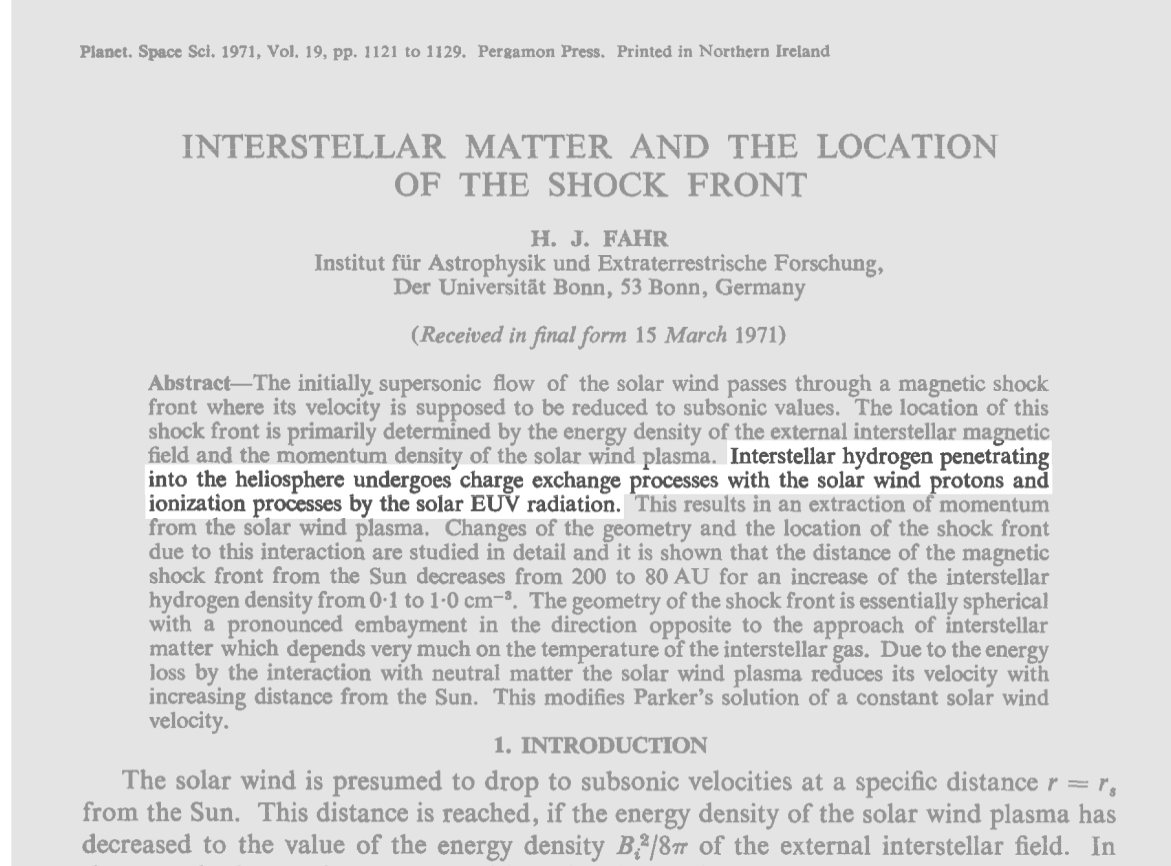
\includegraphics[scale=0.15]{pictures/Screenshot_Fahr_E.png}
			\end{figure}
\end{columns}
\end{frame}
%%%
\begin{frame}{Introduction -- History}
\begin{columns}
	\column{4cm}
		\begin{itemize}
			\item predicted 1971\\ \textbf{Fahr et al.} 
			\item measured 1985\\ \textbf{Moebius et al.} \\ AMPTE/SULEICA
		\end{itemize}
	\column{6.5cm}
		\begin{figure}									
			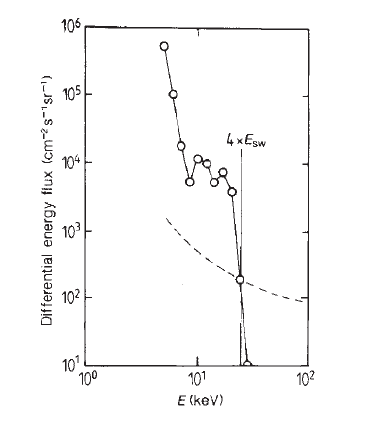
\includegraphics[scale=0.4]{pictures/moebius2_1985.png}
			\caption{$MpQ = 4$, \scriptsize{\textit{Moebius et al. 1985}}}
			\end{figure}
\end{columns}
\end{frame}
%%%
\begin{frame}{Introduction -- Today}
\begin{columns}
	\column{4cm}
		\textbf{Observed PUIs:} \\H\textoverscript{1+}, \textoverscript{3}He\textoverscript{1+}, He\textoverscript{1+}, He\textoverscript{2+}, C\textoverscript{1+}, N\textoverscript{1+}, O\textoverscript{1+}, Ne\textoverscript{1+}, Mg\textoverscript{1+}, Si\textoverscript{1+}, Fe\textoverscript{1+}

		\vspace{0.7cm}
		%
		\textbf{PUI or Solar Wind?}
		\begin{itemize}
			\item Charge state
			\item Velocity distribution function (VDF)
		\end{itemize}
	\column{6cm}
		\flushright
		\begin{figure}
			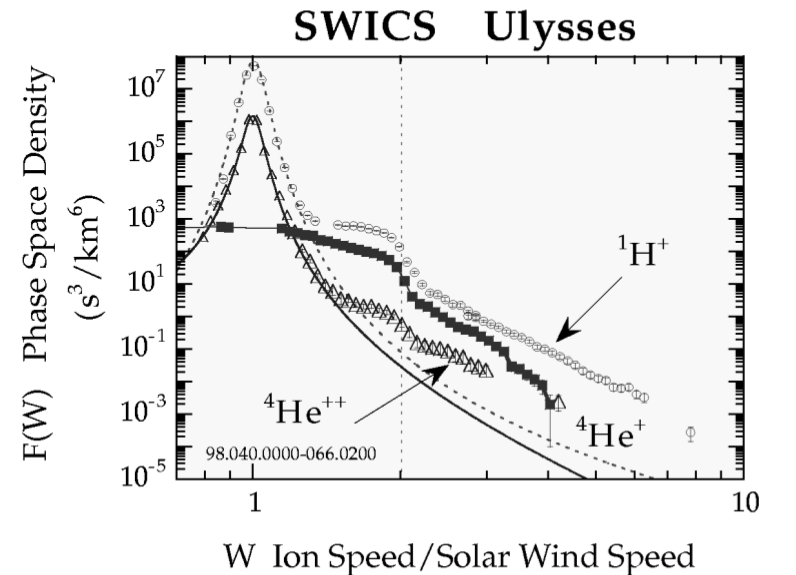
\includegraphics[scale=0.23]{pictures/sw_pui_gloeckler.png}
			\caption{\tiny{\textit{Gloeckler et al. 1999}}}
		\end{figure}
\end{columns}
\end{frame}
%%%
\section{General Concepts}
\begin{frame}{Neutrals from the LISM -- Interstellar PUIs}
	\begin{figure}
		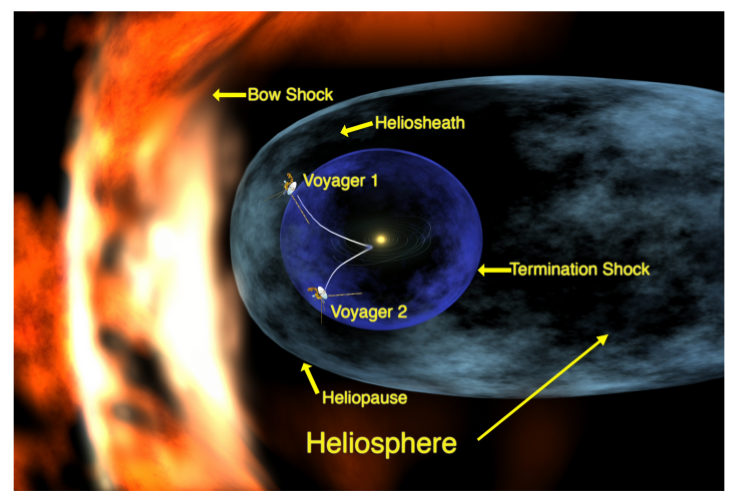
\includegraphics[scale=0.35]{pictures/lism.png}
		\caption{\scriptsize{from \textit{http://science.nasa.gov}}}
	\end{figure}
\end{frame}
%%%
\begin{frame}{Neutrals in the heliosphere}
\begin{figure}
	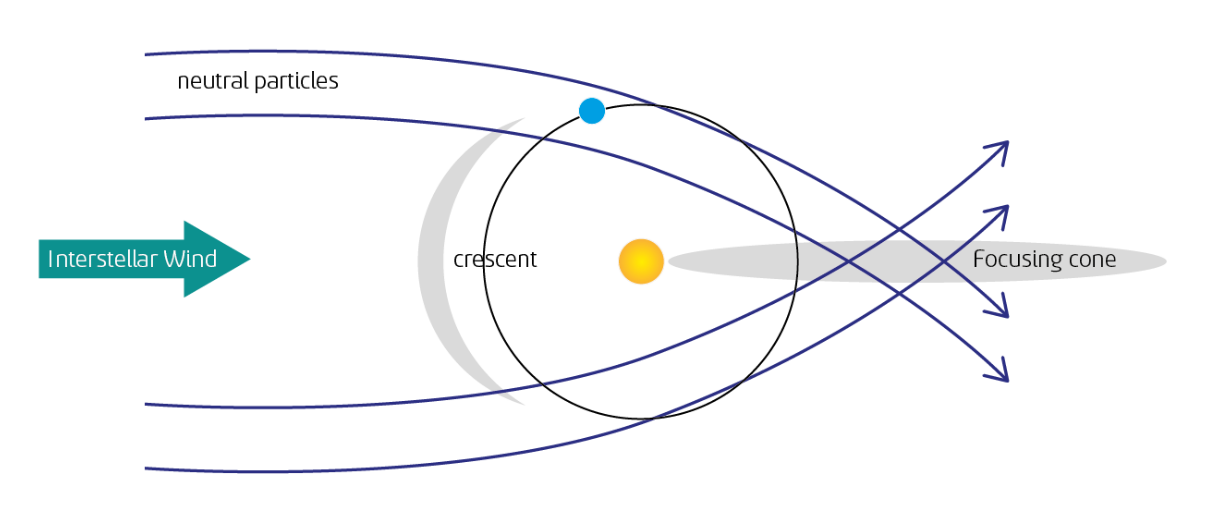
\includegraphics[scale=0.2]{pictures/i_processes_0.png}
	\caption{\tiny{Drews et al., AGU Fall Meeting 2014}}
\end{figure}
\begin{itemize}
	\item Neutrals from LISM enter the heliosphere -- $v_n \approx 25 - 50 \mathrm{km\,s^{-1}}$
	\item subjected to: \\gravitational force, radiation pressure, solar wind particles
\end{itemize}
\end{frame}
%%%
\begin{frame}{Ionisation}
\begin{center}
%Ionisation
\end{center}
\begin{figure}
	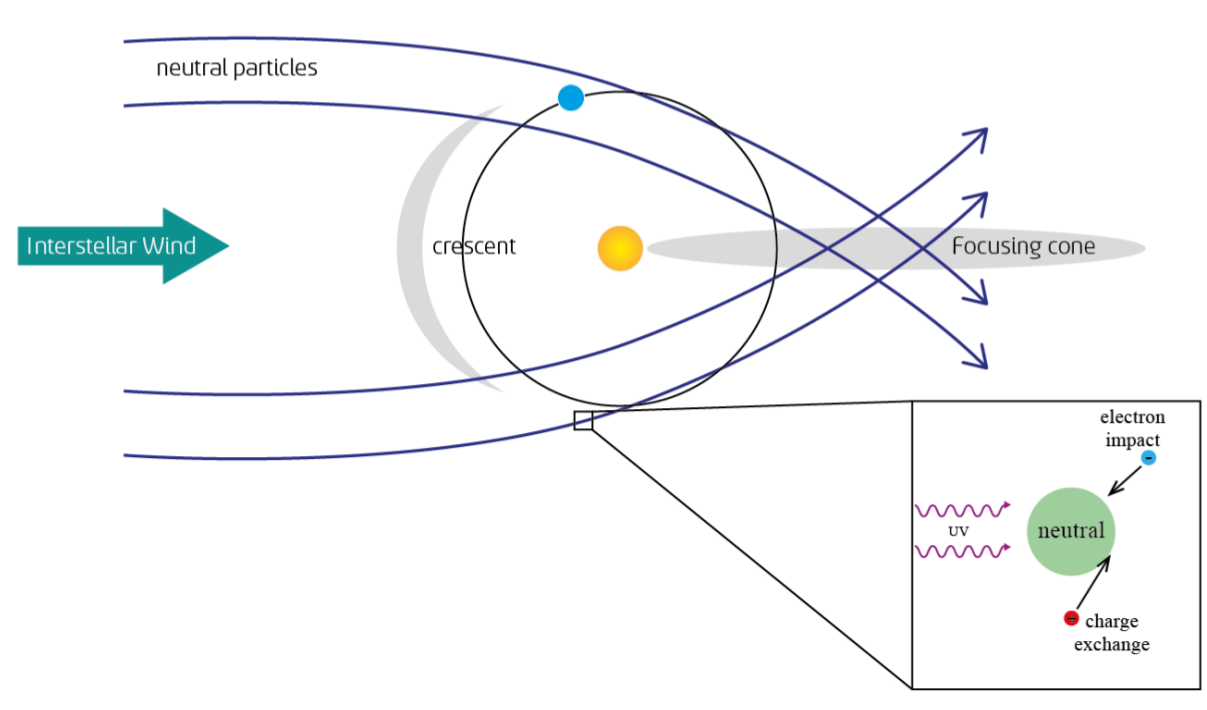
\includegraphics[scale=0.23]{pictures/i_processes_1.png}
	\caption{\tiny{Drews et al., AGU Fall Meeting 2014}}
\end{figure}
\end{frame}
%%%
\begin{frame}{Inner-source PUIs} %1
	\begin{columns}
	\column{5cm}
	\begin{itemize}
		\item \textit{Geiss et al. 1995}: observation of $\mathrm{C^+}$ PUIs
		\vspace{5.0cm}
	\end{itemize}
	\column{6cm}
		\begin{minipage}{5cm}
		\begin{figure}
			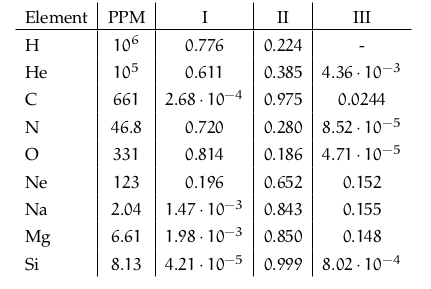
\includegraphics[scale=0.3]{pictures/lism_table.png}
			
			\caption{\scriptsize{Elemental and charge state composition in the LISM\newline Frisch et al. 2011 /  Taut 2018}}
		\end{figure}
		\end{minipage}
	\end{columns}
\end{frame}
%%%
\begin{frame}{Inner-source PUIs} %2
	\begin{columns}
	\column{5cm}
	\begin{itemize}
		\item \textit{Geiss et al. 1995}: observation of $\mathrm{C^+}$ PUIs
		\end{itemize}
		\vspace{0.1cm}
	 \begin{center}
	 Solution: \\ \textbf{Inner source of neutrals} \\
	 $\rightarrow$ Inner-source PUIs
	 \end{center}
	 \begin{itemize}
	 	\item production mechanism: unclear (solar wind $\leftrightarrow$ dust ?)
	 	\item nearly thermalised VDF (peak @ w $\approx$ 1)
	 \end{itemize}
		
	
	\column{6cm}
		\begin{minipage}{5cm}
		\begin{figure}
			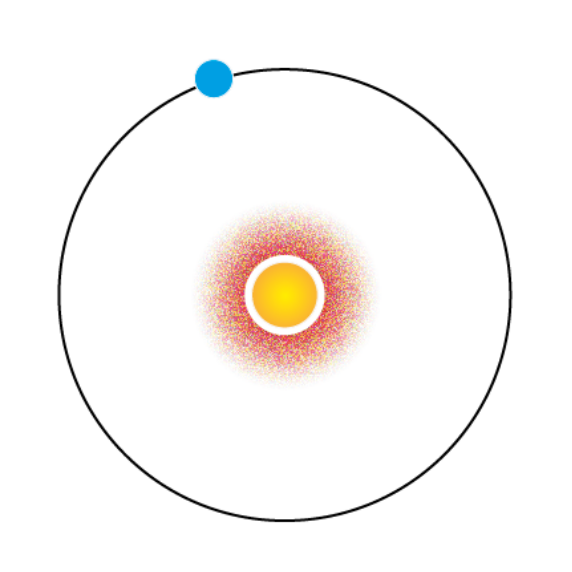
\includegraphics[scale=0.25]{pictures/inner_source.png}
			
			\caption{\scriptsize{2011  Taut 2018}}
		\end{figure}
		\vspace{1cm}
		\end{minipage}
	\end{columns}
\end{frame}
%%%
\begin{frame}{The pickup-process}
\begin{columns}
	\column{4.5cm}
		\flushright
		\begin{figure}
		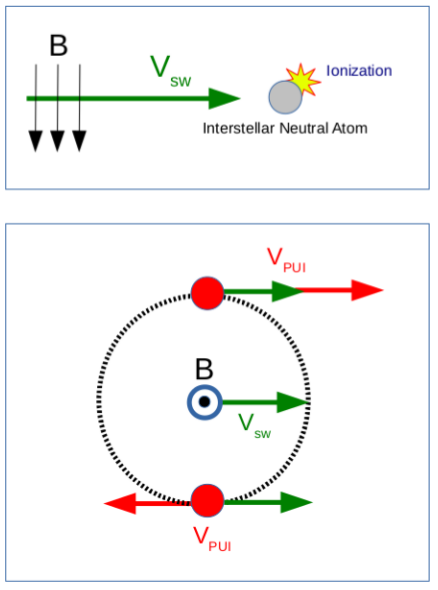
\includegraphics[scale=0.25]{pictures/pu_process_1_2.png}
		\caption{\tiny{Drews et al., AGU Fall Meeting 2014}}
		\end{figure}
	\column{5cm}
	Assumptions:
	\begin{itemize}
		\item particle at rest
		\item $\vec{B} \perp \vec{v}_{SW}$
	\end{itemize}
	\vspace{1cm}
\textbf{	Relative motion \\
	$\rightarrow$ Gyro-motion }
\end{columns}
\end{frame}
%%%
\section{Velocity Distribution Function}
\begin{frame}{Velocity Distribution Function}
\begin{columns}
	\column{4.5cm}
		\flushright
		\begin{figure}
		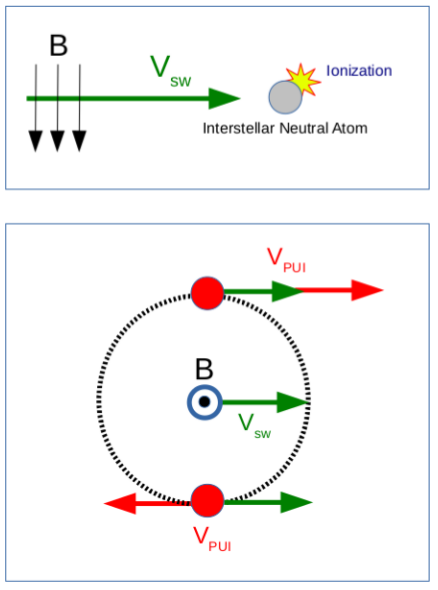
\includegraphics[scale=0.25]{pictures/pu_process_1_2.png}
		\caption{\tiny{Drews et al., AGU Fall Meeting 2014}}
		\end{figure}
	\column{1.5cm}
		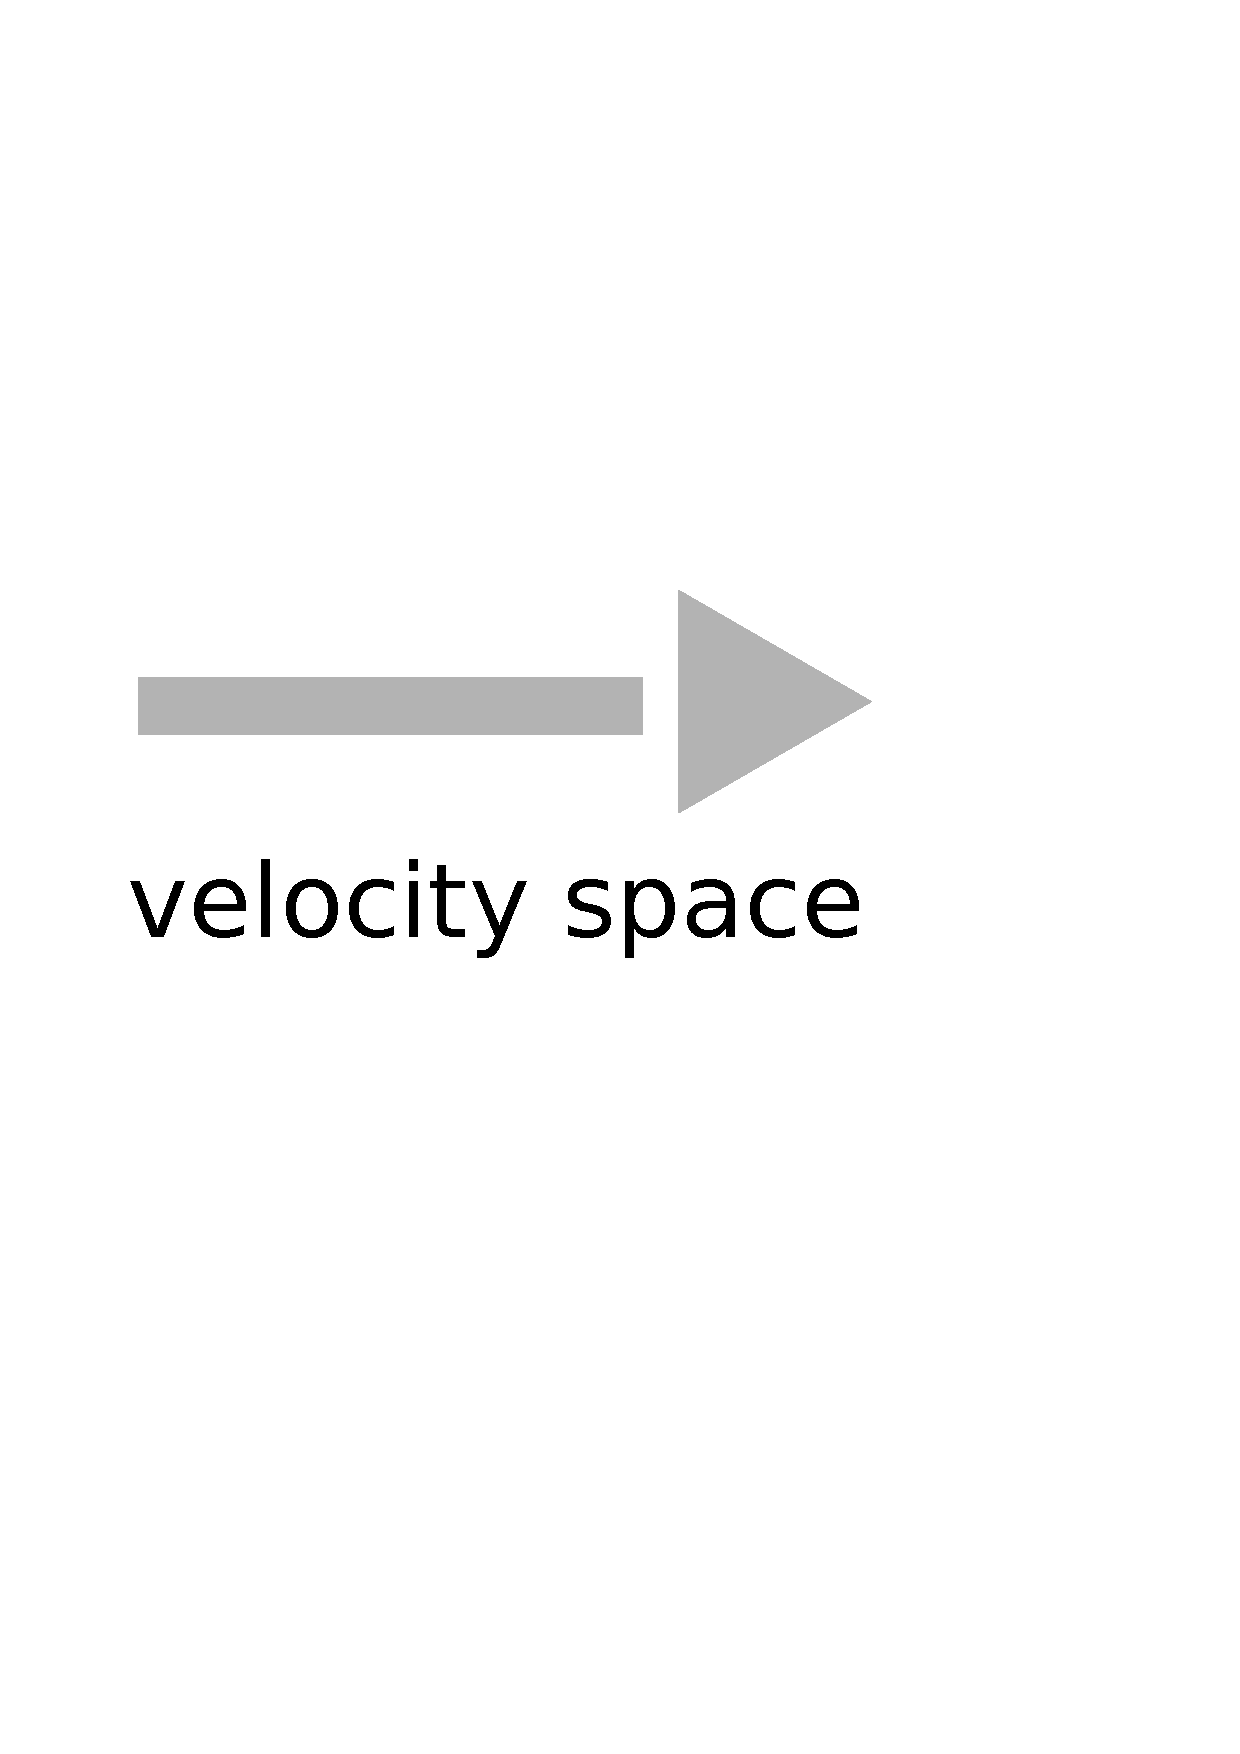
\includegraphics[scale=0.1]{pictures/arrow.pdf}
	\column{5cm}
		\begin{figure}
		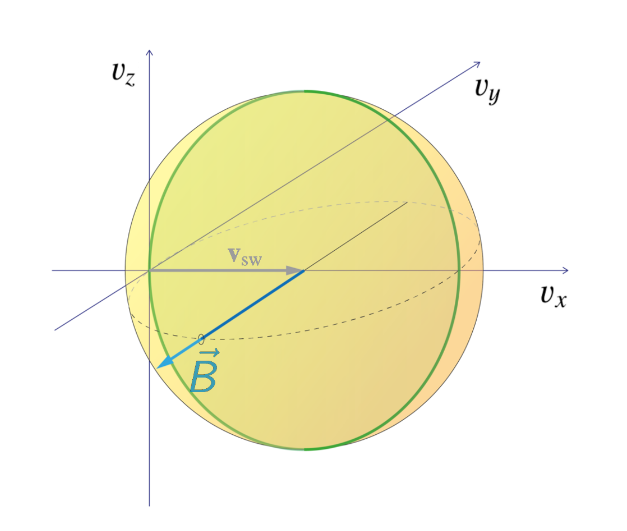
\includegraphics[scale=0.25]{pictures/vdf_3d.png}
		\caption{\tiny{Drews et al., AGU Fall Meeting 2014}}
		\end{figure}
\end{columns}
\end{frame}
%%%
\begin{frame}{Velocity Distribution Function}
	\begin{minipage}{1\textwidth}
	\begin{columns}
	\column{4.5cm}
		\begin{figure}
			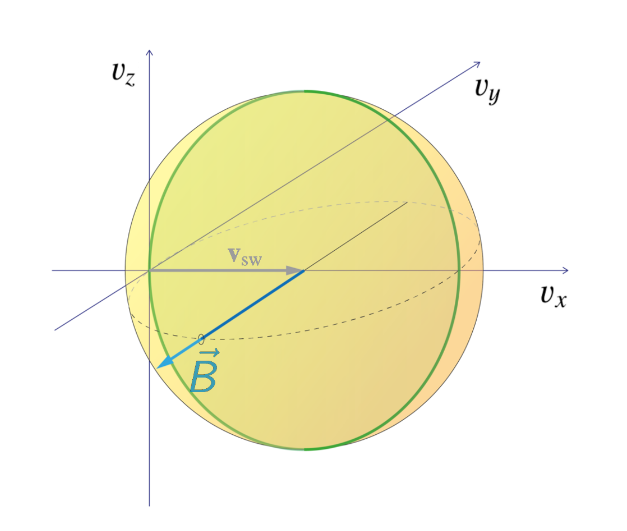
\includegraphics[scale=0.25]{pictures/vdf_3d.png}
			\caption{\tiny{Drews et al., AGU Fall Meeting 2014}}
		\end{figure}
	\column{1.5cm}
		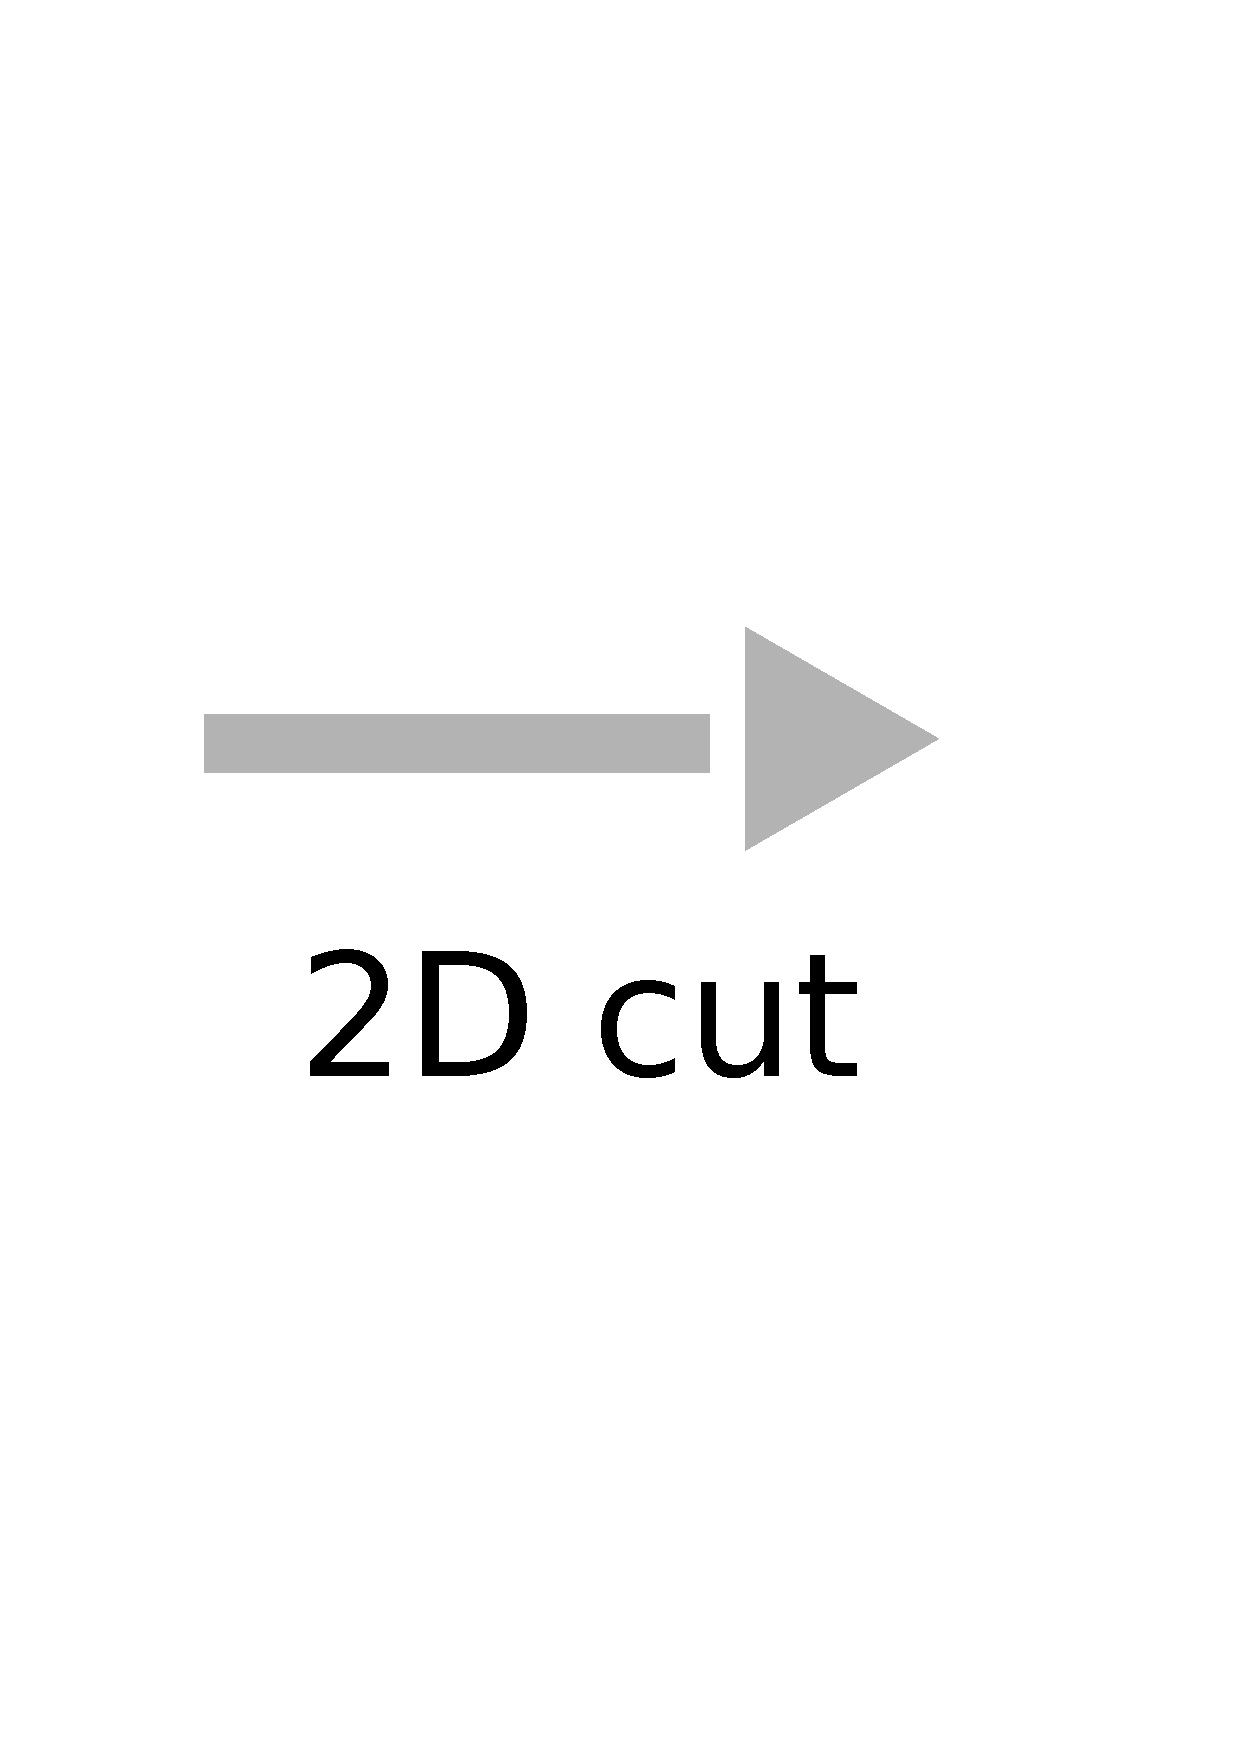
\includegraphics[scale=0.1]{pictures/arrow_2d.pdf}
	\column{5cm}
		\begin{figure}
			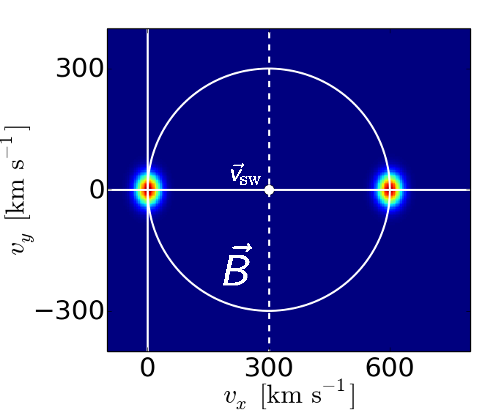
\includegraphics[scale=0.3]{pictures/2d_b.png}
			\caption{\tiny{Taut 2018, disputation}}
		\end{figure}
		%\begin{center}
		%\hspace{0.8cm}$\rightarrow$ cutoff @$2\mathrm{v_{sw}}$
		%\end{center}
	\end{columns}
	\end{minipage}
	\vspace{4cm}
	\begin{minipage}{1\textwidth}
		\vspace{1cm}
		\begin{center}
		%$\longrightarrow$ Injection of PUIs into solar wind: \\ anisotropic torus-shaped VDF
		\end{center}
	\end{minipage}
\end{frame}
%%%
\begin{frame}{Velocity Distribution Function}
	\begin{minipage}{1\textwidth}
	\begin{columns}
	\column{5cm}
		Non-perpendicular $\vec{B}$-field:
		\begin{itemize}
			\item gyro-motion perpendicular to $\vec{B}$
			\item inclination of the torus
			\item[\large{$\Rightarrow$}] \textbf{in SW-frame:} \\ every possible torus is part of a shell with $\mathrm{r} =\mathrm{v_{sw}}$
		\end{itemize}
	\column{5.5cm}
		\begin{figure}
			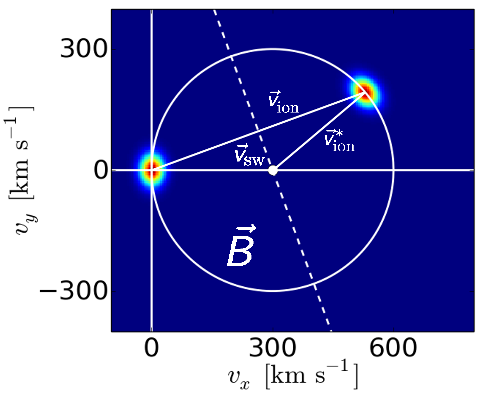
\includegraphics[scale=0.35]{pictures/2d_b_schief.png}
			\caption{\tiny{Taut 2018, disputation}}
		\end{figure}
	\end{columns}
	\end{minipage}
	\vspace{4cm}
	\begin{minipage}{1\textwidth}
		\vspace{.1cm}
		\begin{center}
		$\longrightarrow$ Injection of PUIs into solar wind: \\ anisotropic torus-shaped VDF
		\end{center}
	\end{minipage}
\end{frame}
%%%
\begin{frame}{Velocity Distribution Function}
	\begin{minipage}{1\textwidth}
	\begin{columns}
	\column{5cm}
		Non-perpendicular $\vec{B}$-field:
		\begin{itemize}
			\item gyro-motion perpendicular to $\vec{B}$
			\item inclination of the torus
			\item[\large{$\Rightarrow$}] \textbf{in SW-frame:} \\ every possible torus is part of a shell with $\mathrm{r} =\mathrm{v_{sw}}$
		\end{itemize}
	\column{5.5cm}
		\begin{figure}
			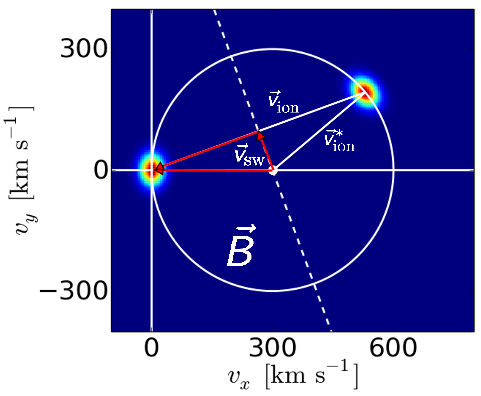
\includegraphics[scale=0.35]{pictures/2d_b_schief_v.png}
			\caption{\tiny{Taut 2018, with modifications}}
		\end{figure}
	\end{columns}
	\end{minipage}
	\vspace{4cm}
	\begin{minipage}{1\textwidth}
		\vspace{.1cm}
		\begin{center}
		$\longrightarrow$ Injection of PUIs into solar wind: \\ anisotropic torus-shaped VDF
		\end{center}
	\end{minipage}
\end{frame}
%%%
\begin{frame}{Velocity Distribution Function -- measurement}
	\begin{columns}
	\column{6.5cm}
		\begin{figure}
			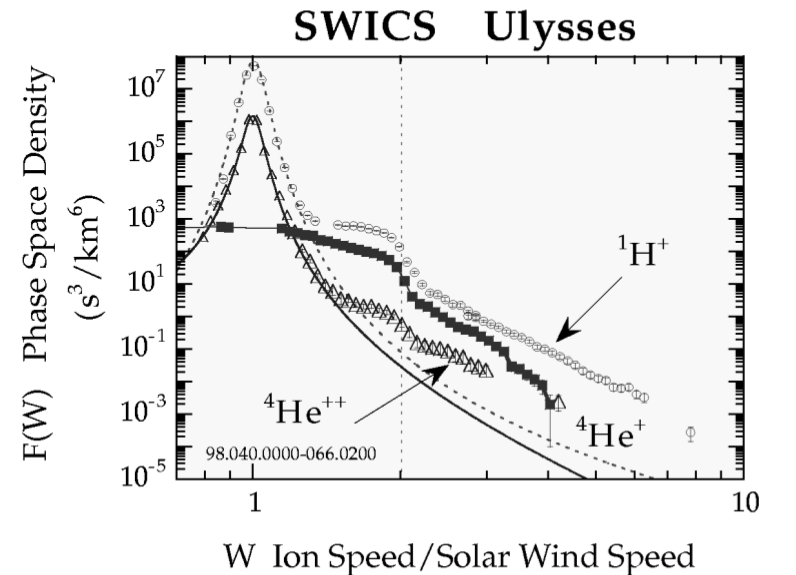
\includegraphics[scale=0.28]{pictures/sw_pui_gloeckler.png}
			\caption{\tiny{\textit{Gloeckler et al. 1999}}}
		\end{figure}
	\column{4.cm}
		\begin{center}
		Reminder:
		\end{center}
		\begin{figure}
			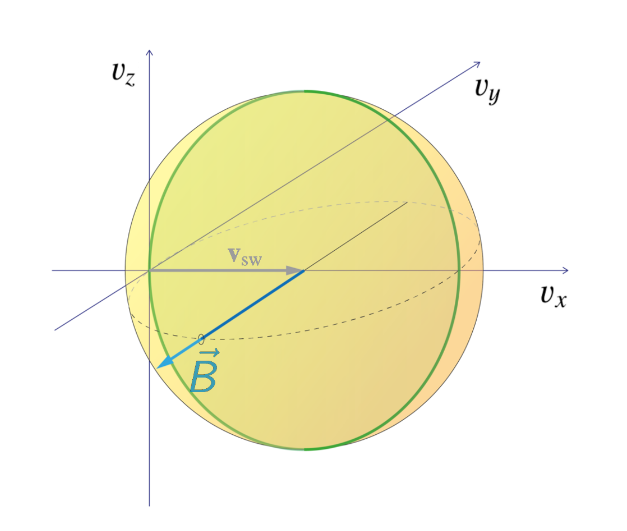
\includegraphics[scale=0.15]{pictures/vdf_3d.png}
		\end{figure}
		\vspace{1cm}
	\end{columns}
\end{frame}
%%%
\begin{frame}{Velocity Distribution Function -- Diffusion} %1
\begin{columns}
	\column{5cm}
		\begin{itemize}
			\item Pitch-angle scattering 
			\vspace{1cm}
			\item<alert> Deceleration processes (\textit{``cooling''})
			\vspace{1cm}
			\item<alert> Acceleration processes
		\end{itemize}
	\column{7.5cm}
		\begin{figure}
			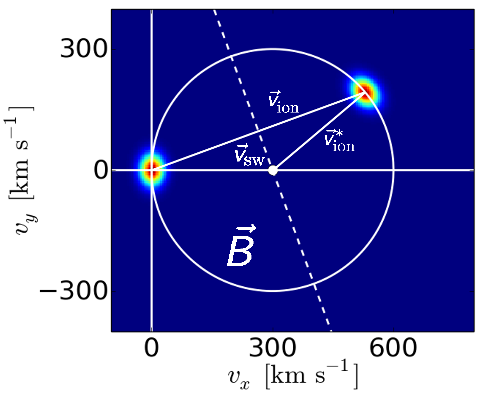
\includegraphics[scale=0.3]{pictures/2d_b_schief.png}
			\caption{\tiny{Taut 2018, disputation}}
		\end{figure}
\begin{center}
	   \textit{Vasyliunas $\&$ Siscoe 1978}: \\$\rightarrow$ fast isotropisation
\end{center}
\end{columns}
\end{frame}
%%%
\begin{frame}{Velocity Distribution Function -- Diffusion} %1
\begin{columns}
	\column{5cm}
		\begin{itemize}
			\item Pitch-angle scattering 
			\vspace{1cm}
			\item<alert> Deceleration processes (\textit{``cooling''})
			\vspace{1cm}
			\item<alert> Acceleration processes
		\end{itemize}
	\column{7.5cm}
		\begin{figure}
			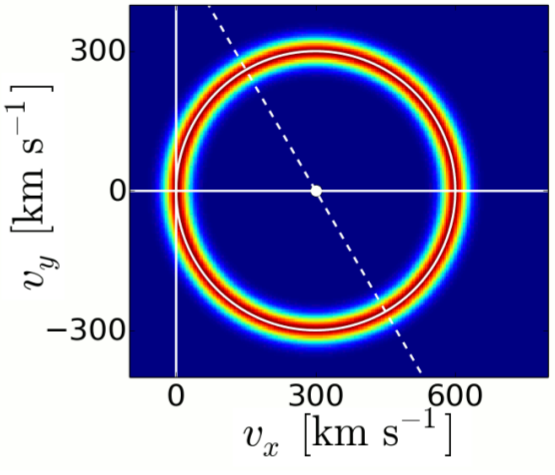
\includegraphics[scale=0.26]{pictures/pa.png}
			\caption{\tiny{Taut 2018, disputation}}
		\end{figure}
\begin{center}
	   \textit{Vasyliunas $\&$ Siscoe 1978}: \\$\rightarrow$ fast isotropisation
\end{center}
\end{columns}
\end{frame}
%%%
\begin{frame}{Velocity Distribution Function -- Diffusion} %2
\begin{columns}
	\column{5cm}
		\begin{itemize}
			\item Pitch-angle scattering 
			\vspace{1cm}
			\item<alert> Deceleration processes (\textit{``cooling''})
			\vspace{1cm}
			\item<alert> Acceleration processes
		\end{itemize}
	\column{7.5cm}
		\begin{figure}
			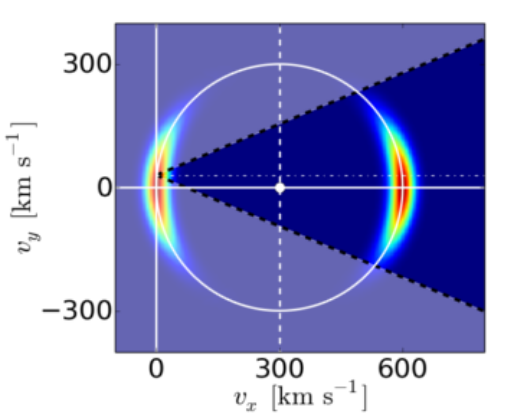
\includegraphics[scale=0.15]{pictures/fov.png} \\
			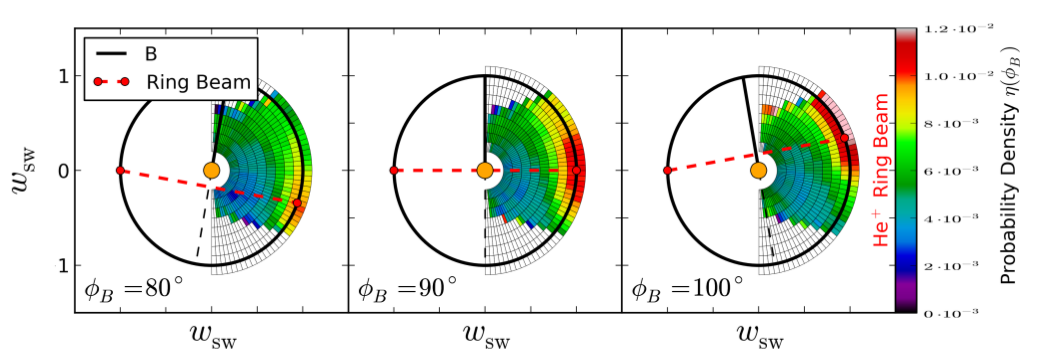
\includegraphics[scale=0.2]{pictures/rvdf}
			\caption{\scriptsize{Drews et al. 2015}}
		\end{figure}
\begin{center}
		\begin{tabular}{@{}l@{}}
			\tabitem anisotropic feature \\
			\tabitem $\vec{B}$-dependency
		\end{tabular}
\end{center}
\end{columns}
\end{frame}
%%%
\begin{frame}{Velocity Distribution Function -- Diffusion} %3
\begin{columns}
	\column{5cm}
		\begin{itemize}
			\item Pitch-angle scattering 
			\vspace{1cm}
			\item Deceleration processes (\textit{``cooling''})
			\vspace{1cm}
			\item<alert> Acceleration processes
		\end{itemize}
	\column{7.5cm}
		\begin{figure}
			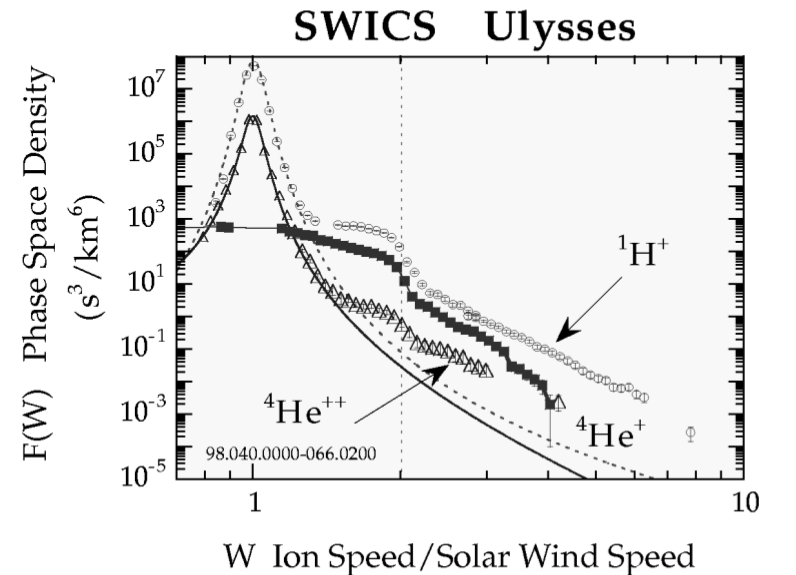
\includegraphics[scale=0.2]{pictures/sw_pui_gloeckler.png}
			\caption{\tiny{\textit{Gloeckler et al. 1999}}}
		\end{figure}
		\[E^{\frac{3}{4}}r = const.\]
		\[r_0=\left({\frac{E}{E_{0}}}\right)^{\frac{3}{4}}r\]
\end{columns}
\end{frame}
%%%
\begin{frame}{Velocity Distribution Function -- Diffusion} %4
\begin{columns}
	\column{5cm}
		\begin{itemize}
			\item Pitch-angle scattering 
			\vspace{1cm}
			\item Deceleration processes (\textit{``cooling''})
			\vspace{1cm}
			\item Acceleration processes
		\end{itemize}
	\column{7.5cm}
		\begin{figure}
			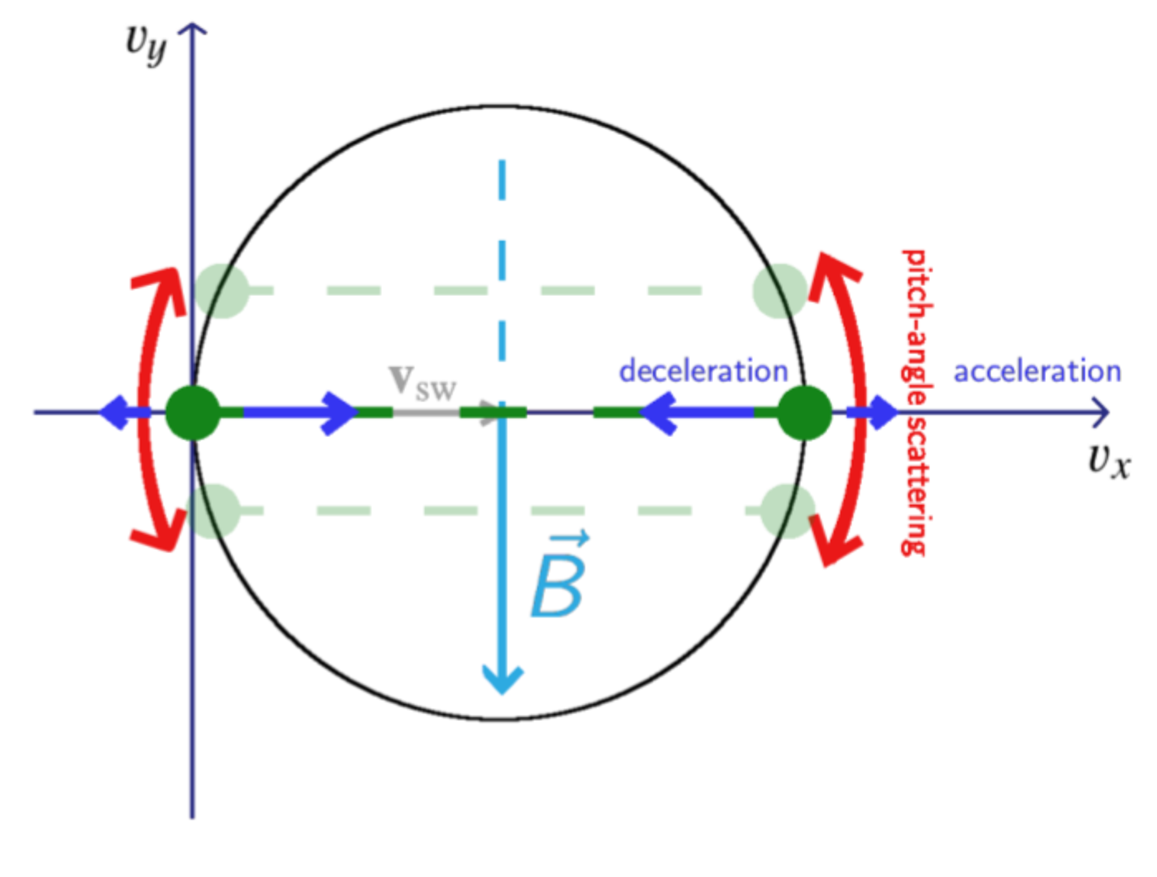
\includegraphics[scale=0.25]{pictures/mods2.pdf}
			\caption{\scriptsize{Taut et al., UNH Space Science Seminar 2017}}
		\end{figure}
\end{columns}
\end{frame}
%%%
\section{Outlook}
\begin{frame}{Outlook}
\begin{columns}
	\column{2.5cm}
		\begin{figure}
			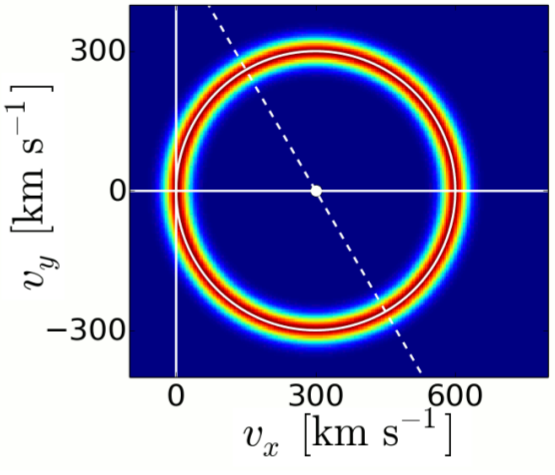
\includegraphics[scale=0.15]{pictures/pa.png}
		\end{figure}
	\column{1cm}
	\vspace{1cm}
		\hspace{2.5cm}
		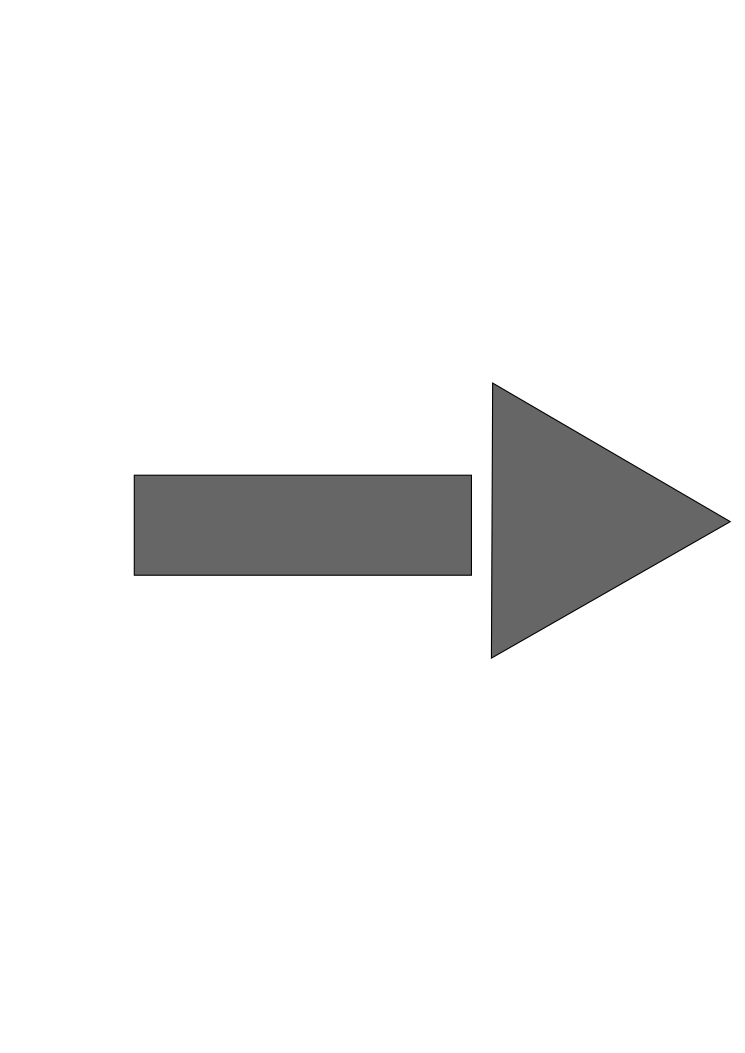
\includegraphics[scale=0.05]{pictures/pfeil_normal.png}
	\column{5.8cm}
		\begin{figure}
			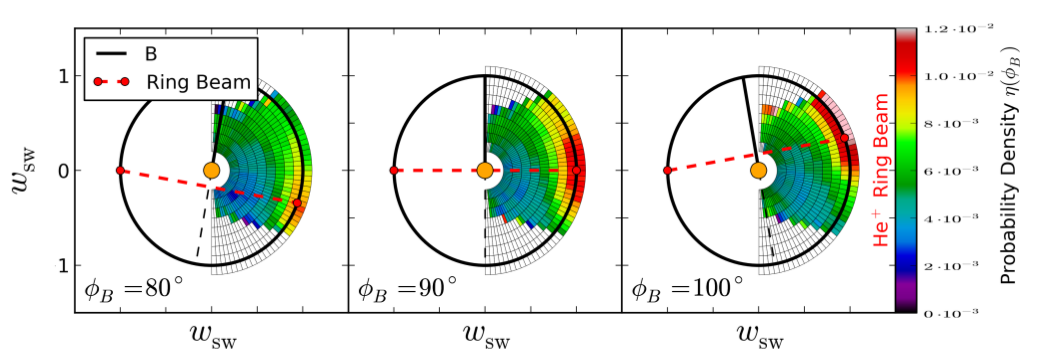
\includegraphics[scale=0.17]{pictures/rvdf}
		\end{figure}
\end{columns}
\begin{columns}
	\column{7cm}
	\begin{figure}[h]
		\centering
		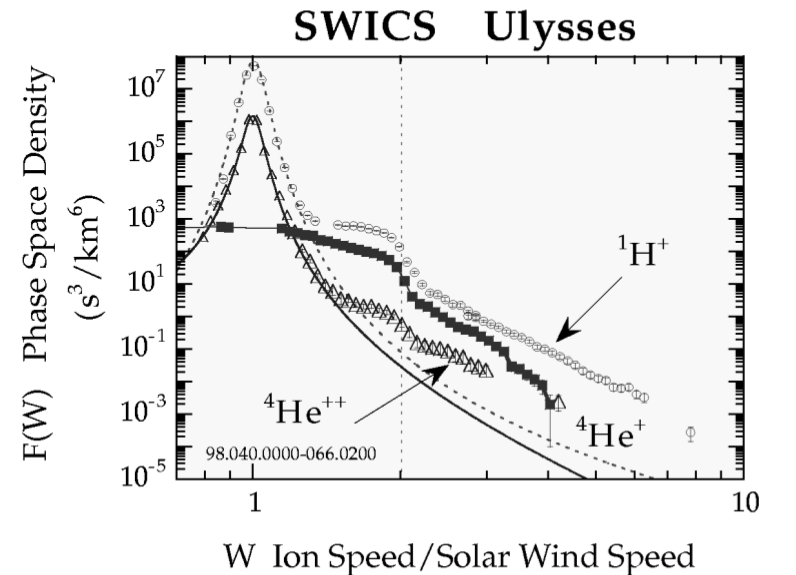
\includegraphics[scale=0.22]{pictures/sw_pui_gloeckler.png}
		\begin{center}
			\caption{\tiny{\textit{Gloeckler et al. 1999}}}
		\end{center}
	\end{figure}
		\column{4cm}
\begin{center}	
		\textbf{How does the VDF evolve after injection?}
\end{center}
		\vspace{3.5cm}
\end{columns}
\end{frame}
%%%
\begin{frame}{Outlook}
	\begin{columns}
		\column{6cm}
		\flushleft
		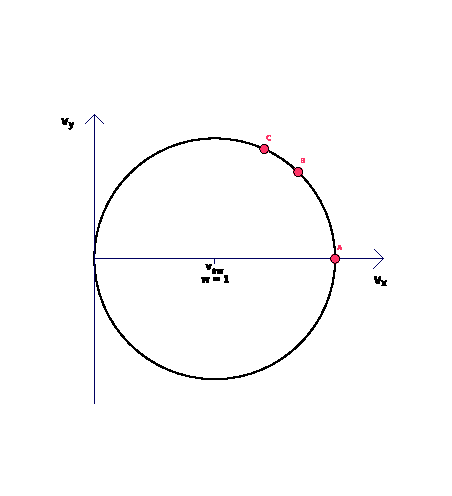
\includegraphics[scale=0.9]{pictures/detektor11.pdf}
		\column{5cm}
		\begin{figure}
		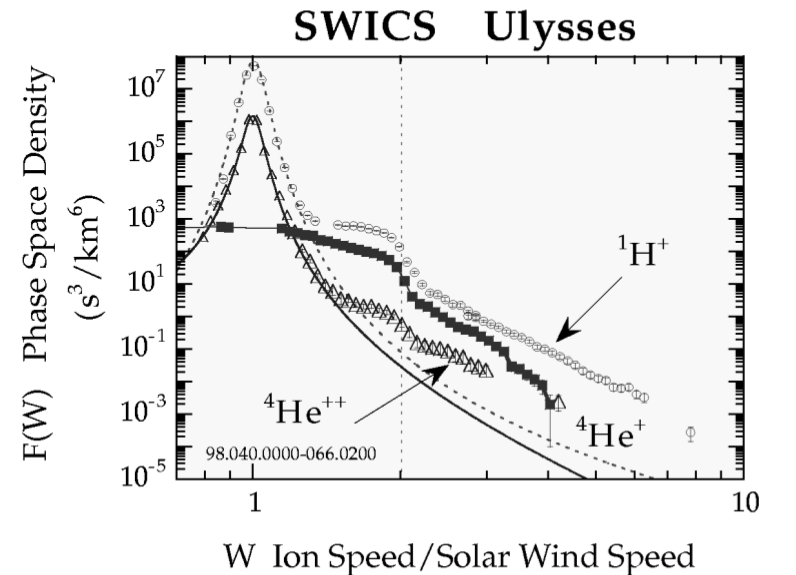
\includegraphics[scale=0.18]{pictures/sw_pui_gloeckler.png}
		\caption{\tiny{\textit{Gloeckler et al. 1999}}}		
		\end{figure}
			Assumption: \\Particles on the shell \\with $r = v_{sw}$
	\end{columns}
\end{frame}
%%%
\begin{frame}{Outlook}
	\begin{columns}
		\column{6cm}
		\flushleft
		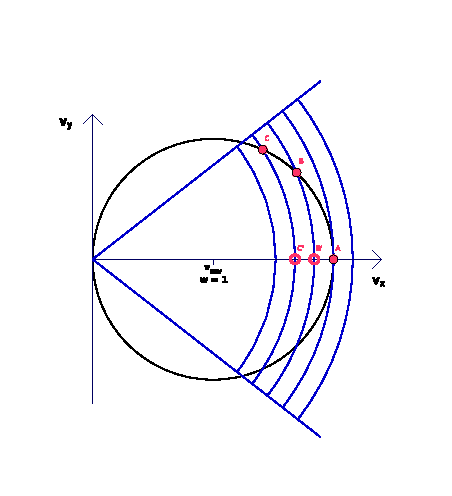
\includegraphics[scale=0.9]{pictures/detektor22.pdf}
		\column{5cm}
		\begin{figure}
		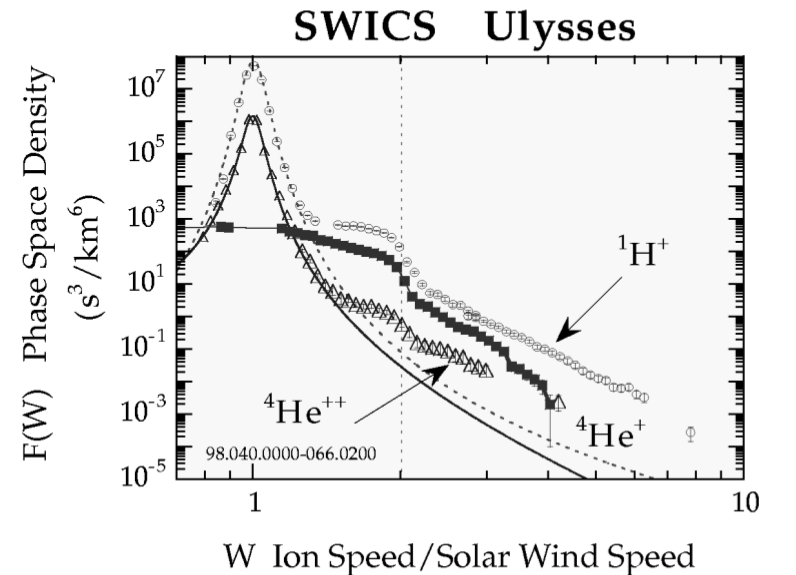
\includegraphics[scale=0.18]{pictures/sw_pui_gloeckler.png}
		\caption{\tiny{\textit{Gloeckler et al. 1999}}}		
		\end{figure}
		Detector integrates over every shell:
		\[w = \frac{v_x}{v_{sw}}\]
	\end{columns}
\end{frame}
%%%
\begin{frame}{Outlook}
	\begin{columns}
		\column{6cm}
		\flushleft
		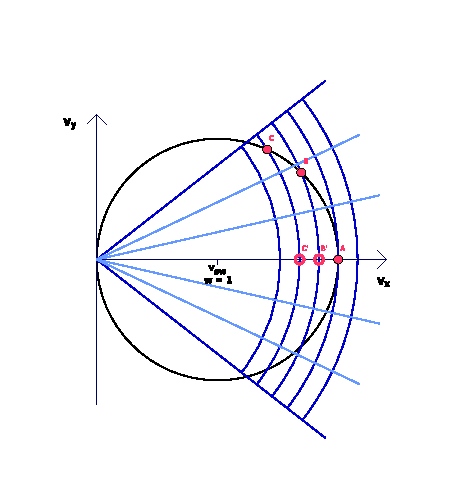
\includegraphics[scale=0.9]{pictures/detektor3.pdf}
		\column{5cm}
		\begin{figure}
		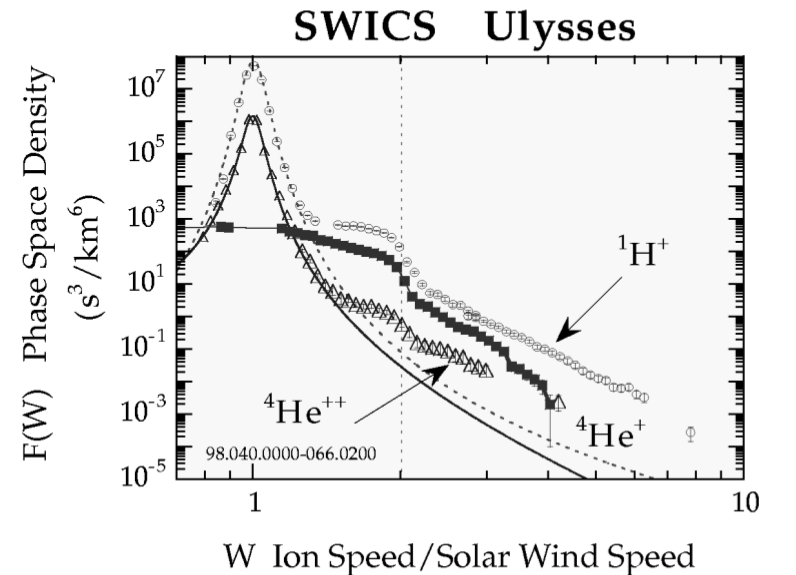
\includegraphics[scale=0.18]{pictures/sw_pui_gloeckler.png}	
		\end{figure}
		\begin{columns}
		\column{3.5cm}
		Ulysses/SWICS: \\detector can distinguish between segments on one shell
		\column{1.5cm}
		\end{columns}
		
	\end{columns}
\end{frame}
%%%
\begin{frame}{Outlook}
	\begin{columns}
		\column{6cm}
		\flushleft
		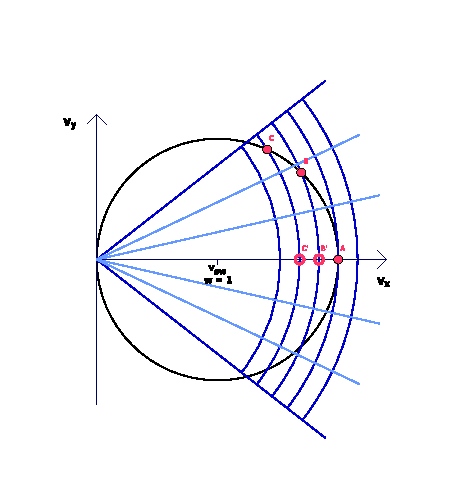
\includegraphics[scale=0.9]{pictures/detektor3.pdf}
		\column{5cm}
		\begin{figure}
		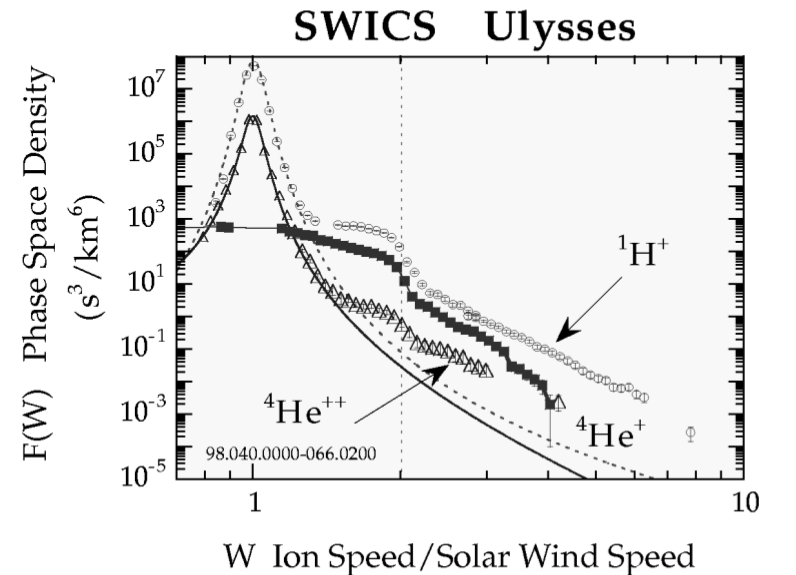
\includegraphics[scale=0.18]{pictures/sw_pui_gloeckler.png}	
		\end{figure}
		\begin{columns}
		\column{3.5cm}
		Ulysses/SWICS: \\detector can distinguish between segments on one shell
		\column{1.5cm}
		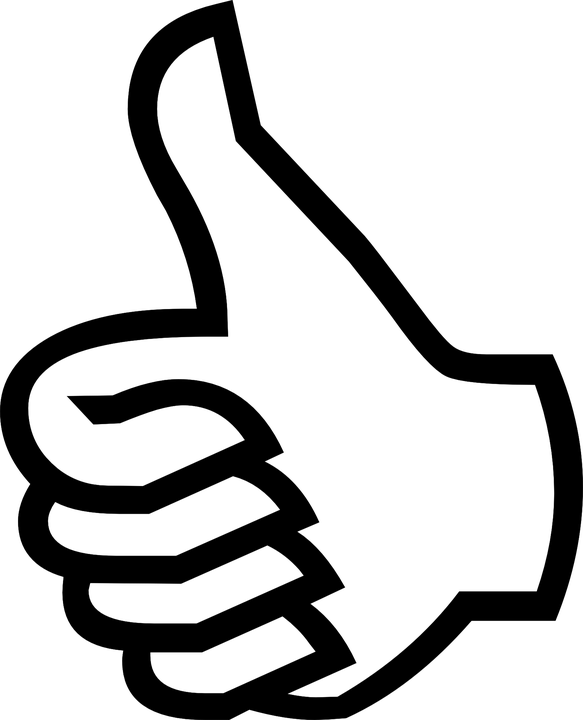
\includegraphics[scale=0.05]{pictures/thumbsup.png}
		\end{columns}
		
	\end{columns}
\end{frame}
%%%
\begin{frame}{Pickup Ions -- Anne Fischer -- Conclusion}
\begin{itemize}
	\item Introduction to Pickup ions and their basic concepts: \\
	sources, pickup-process
	\vspace{1cm}
	\item Velocity distribution: models and measurements
	\vspace{1cm}
	\item How 2D-measurements can help to understand processes better
\end{itemize}
\end{frame}
%
%
%
\end{document}